\documentclass[11pt]{article}
\usepackage[preprint]{acl}
\usepackage{times}
\usepackage{latexsym}
\usepackage[T1]{fontenc}
\usepackage[utf8]{inputenc}
\usepackage{microtype}
\IfFileExists{inconsolata.sty}{\usepackage{inconsolata}}{}  %
\usepackage{booktabs}
\usepackage{tabularx}
\usepackage{amsmath}
\usepackage{pgfplots}
\pgfplotsset{compat=1.17}

\usepackage{url}
\newcommand{\paperauthor}{Atila Vahedian}
\newcommand{\paperaffil}{Independent researcher}
\newcommand{\releaseurl}{\url{https://github.com/atilavahedian/babylm-gap}}

\title{Where the 10M-Word Gap Lives: Noise, Unlearned Structure and Missing\\ Information in BabyLM Data Efficiency}

\author{\paperauthor \\ \paperaffil}

\begin{document}
\maketitle

\begin{abstract}
A language model trained on 10M words falls 0.715 nats/word (calibrated) short of a model of the same size trained on
100M words. We ask where that gap lives and how much of it a learner that sees only 10M words could close under the
BabyLM 2025 strict-small rules. Using seed ensembles and a distillation oracle on the same held-out words, we split the
raw gap between 10-epoch 10M models and the 100M model, 0.74 nats/word, into single-model noise (0.29, the gain of an
8-model ensemble), an upper bound on structure that is in the 10M words but unlearned (0.23), and a lower bound on
information that 10M words do not contain (0.22). A perfect legal learner could therefore gain at most about 4$\times$
in data-equivalent terms, and 10$\times$ is not in the data. The 100M model was not tuned at 100M; a better one would
widen the gap, raising the absent part and lowering the ceiling. We then report ten pre-registered attacks on the gap,
all of which failed, and one measured point: a two-model ensemble, a known technique, beats the best single model of
equal compute by 0.086 nats/word at 28 layers (at least 1.22$\times$ data-equivalent), and the gain holds across two
sizes. On the official BabyLM zero-shot suite, however, this gain does not clear the seed-noise bar, and our best model
scores below the published GPT-BERT causal-focus baseline (38.97 vs 40.32 on the composite with reading rescored). All
bars were registered before the results they judged, except two disclosed rules that only tightened them.
\end{abstract}

\section{Introduction}
Humans learn language from roughly 10--100M words; language models typically need orders of magnitude more. The BabyLM
challenge \citep{babylm2025} turns this into a controlled question: how good a model can one train on 10M words? Most
entries propose a method and report whether a benchmark score went up. We take a different angle and first measure the
target. How large is the gap between the same model trained on 10M and on 100M words, what is it made of, and how much of it is
reachable at all by a learner that only sees 10M words?

We answer with a gap map on held-out words. Averaging eight seeds of the 10M model measures how much of the gap is
single-model noise. A student trained on the 10M contexts to match a 100M-word teacher bounds how much is structure
present in the 10M words but unlearned. What even that student cannot recover is information the 10M words do not
contain. The gap splits into noise, an upper bound on learnable structure, and a lower bound on absent information,
which caps any legal learner at about 4$\times$ data-equivalent efficiency on this data.

The map then explains a run of negative results. We tested ten attacks under pre-registered kill lines: noise
regularisers, subword dropout, self-generated contexts, ensemble distillation, shared-trunk and heterogeneous ensembles,
wider models, heavy weight decay and looped depth. None cleared its bar once calibrated or compared at equal compute. The one
lever that held is old: averaging two models trained on the same data. It attacks only the noise part of the gap, gives
at least 1.22$\times$ (point 1.32) at equal compute on DEV loss at 28 layers, and does not move the official zero-shot scores beyond seed noise.

Our contributions are measurements, not new methods: (1) a decomposition of the 10M-to-100M gap into noise, an upper
bound on learnable structure, and a lower bound on absent information; (2) a ceiling for any legal learner on this data; (3) a set of
pre-registered, compute-matched negative results; and (4) a replication of the seed-ensemble gain at two sizes, with
its official-benchmark tie. Every comparison bar was registered by an independent automated reviewer that wrote no
model code, before the result it judged (Section~\ref{sec:setup}).

\section{Related work}
\label{sec:related}
\paragraph{BabyLM.} The BabyLM challenge fixes the training data at 10M or 100M words and compares learners on a shared
evaluation suite \citep{babylm2025}. Hybrid causal and masked objectives such as GPT-BERT \citep{charpentier2024gptbert}
are among the strongest entries and serve as our published reference point. Distilling an ensemble of teachers trained
on the same small corpus into one student was shown to work by \citet{timiryasov2023babyllama}; our attack 5 revisits
it under an exposure cap that counts the teachers' training.

\paragraph{Ensembles under a fixed data budget.} Deep ensembles of independently seeded models improve likelihood and
calibration \citep{lakshminarayanan2017}, and members trained with different recipes decorrelate their errors somewhat
more than seeds alone \citep{gontijolopes2022}. \citet{kim2025infinite} study pre-training when data, not compute, is
the limit, and find that heavy regularisation and ensembling, followed by distillation, make better use of a fixed
corpus. Our two-model result is a replication of this known idea at BabyLM scale, under its exposure rule.

\paragraph{Repetition and data-constrained scaling.} \citet{hoffmann2022chinchilla} give compute-optimal trade-offs when
data is plentiful; \citet{muennighoff2023scaling} show that repeated epochs lose value quickly beyond a few passes. Our
data-wall probe (Section~\ref{sec:rung0}) asks the same question for a 10M-word corpus at 16 epochs.

\paragraph{Looped depth.} Running a block of layers several times with shared weights trades parameters for compute
\citep{chen2026looped,parcae2026,ouro2025}. At equal FLOPs on our data it lost to a plain deeper model.

\section{Setup}
\label{sec:setup}
We measure how far a model trained on 10M words falls short of a model of the same size trained on 100M words, and what closes
that gap under BabyLM 2025 strict-small rules \citep{babylm2025}.

\paragraph{Track and rules.} At most 10M unique words, at most 10 epochs, and at most 100M words of total exposure,
counting every model's exposure (teachers and generators included); no outside pretrained weights. EWoK
\citep{ivanova2024ewok} is evaluation-only.

\paragraph{Base model.} A 12-layer, 384-wide causal Transformer (size S) adapted from the modded-nanogpt recipe
\citep{jordan2024moddednanogpt}: tied output layer, no value-embedding tables, weight decay 0.4, Muon optimiser
\citep{jordan2024muon}. Six epochs beat ten by 0.039 nats/word raw (0.020 calibrated), so the base trains for 6 epochs (E6).

\paragraph{Reference.} The E6 pool: 5 seeds, torch 2.7, solo runs; mean 4.9693 nats/word raw (SD 0.0057).

\paragraph{Metric.} Nats per whitespace word on the full DEV set, with blank lines as document breaks. Claims use a
calibrated score, cal\_t (``calibrated''): temperature scaling \citep{guo2017calibration} jointly with a mixture weight $\lambda$ toward the training unigram distribution, both cross-fitted on DEV document
parity. Every claim must pass on two legs: full DEV, and a guarded DEV that drops the 10,277 words containing a
character never seen in training.

\paragraph{Claim floor.} Two pool SDs on cal\_t: 0.0111 (full) / 0.0065 (guarded). Packed-vs-solo and torch
2.7-vs-2.9 systematics are about 0.012 each, so claims use solo runs in one environment.

\paragraph{Yardstick.} $x = 10^{\,\mathrm{gain}/Y}$, a DEV-loss data-equivalent multiplier that assumes log-linear
returns to data. $Y$ is our 10M reference (5 seeds) minus our best 100M point (3 seeds) on cal\_t: $Y = 0.715$ / 0.690
nats/word (full / guarded; Welch 95\% [0.708, 0.722] / [0.686, 0.695]), so 2$\times$ needs a gain of 0.215 / 0.208.
The 100M point is the same 12-layer model with the original recipe's settings (no weight decay, untied output, value
embeddings, 10 epochs), because our 10M settings underfit at 100M. It is the best we hold, not one tuned at 100M, so every $x$ is an upper bound. We quote the lower end of
its 95\% interval (the gain's spread, df 2, reference spread included), taking the smaller of full DEV and DEV with the
134,739 words of lines that also occur verbatim in the 100M corpus removed.

\paragraph{Pre-registration.} An independent automated reviewer that wrote no model code registered
every bar before the result it judged and could veto a claim. Two rules, the calibrated score and the never-seen-character
guard, were added after the raw screen number of attack 1 (Table~\ref{tab:failed}) had been seen; both only tightened
bars and applied to every comparison.

\section{The map: where the gap lives}
\label{sec:map}
The raw gap between 10-epoch 10M models and the 100M model, 0.743 nats/word, splits into noise, an upper bound on
learnable structure, and a lower bound on absent information: single-model noise (0.29 nats/word), an upper bound on
structure that is in the data but unlearned (0.23), and a lower bound on information absent from 10M words (0.22). The
100M model was not tuned at 100M (Section~\ref{sec:setup}). A better one would widen the gap, so on that axis the
absent slice is a lower bound and the ceiling of Section~\ref{sec:ceiling} an upper bound. Three probes measure the
parts on the same DEV words:
\begin{itemize}
\item \textbf{Noise (posterior variance), lower bound.} Eight seeds of the 10M model, averaged: the mean member minus
  the 8-model mixture. This is the gain of an 8-model ensemble, a lower bound on posterior variance: the $(1 - 1/K)$
  rule puts the limit near 0.33, and the extra $\sim$0.04 comes out of the learnable slice, which is measured from the
  8-model mixture.
\item \textbf{Learnable-but-unlearned, upper bound.} A student on the 10M contexts trained to match a 100M teacher's
  predictions (the C1-oracle) closes $\sim$70\% of the gap. The 8-model mixture minus this oracle bounds what any 10M
  learner could still extract.
\item \textbf{Absent information, lower bound.} The oracle minus the 100M model itself: what no student reading only
  10M contexts recovers.
\end{itemize}

\begin{table}[t]
\centering
\small
\begin{tabular}{lrr}
\toprule
Part & nats/word & share \\
\midrule
Single-model noise (8 seeds) & 0.289 & 39\% \\
Learnable, upper bound & 0.233 & 31\% \\
Absent, lower bound & 0.221 & 30\% \\
\midrule
Measured gap & 0.743 & \\
\bottomrule
\end{tabular}
\caption{The three parts of the gap (raw leg; 10M members and student in torch 2.9.1, the 100M model in torch 2.7,
whose shift is at most $\sim$0.012). Members are 10-epoch seeds, so the measured gap
is 0.74, close to the calibrated $Y$ of 0.715. Guarded leg: 0.282 / 0.231 / 0.202.}
\label{tab:map}
\end{table}

\begin{figure}[t]
\centering
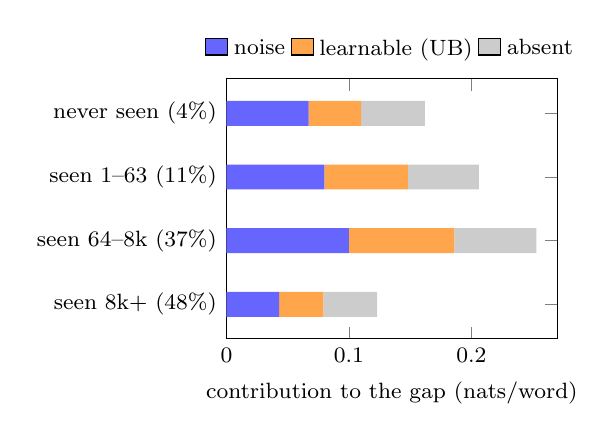
\begin{tikzpicture}
\begin{axis}[
  xbar stacked, scale only axis, width=4.2cm, height=3.3cm, bar width=9pt,
  xmin=0, xmax=0.27, xtick={0,0.1,0.2}, scaled x ticks=false,
  xticklabel style={/pgf/number format/fixed, /pgf/number format/precision=2},
  xlabel={contribution to the gap (nats/word)},
  symbolic y coords={8k+,64-8k,1-63,0}, ytick=data, y dir=normal,
  yticklabels={{seen 8k+ (48\%)},{seen 64--8k (37\%)},{seen 1--63 (11\%)},{never seen (4\%)}},
  yticklabel style={font=\footnotesize}, tick label style={font=\footnotesize},
  xlabel style={font=\footnotesize},
  legend style={font=\footnotesize, at={(0.5,1.03)}, anchor=south, legend columns=3, draw=none},
  enlarge y limits=0.18,
]
\addplot[fill=blue!60, draw=none] coordinates {(0.043,8k+) (0.100,64-8k) (0.080,1-63) (0.067,0)};
\addplot[fill=orange!70, draw=none] coordinates {(0.036,8k+) (0.086,64-8k) (0.068,1-63) (0.043,0)};
\addplot[fill=gray!40, draw=none] coordinates {(0.044,8k+) (0.067,64-8k) (0.058,1-63) (0.052,0)};
\legend{noise, learnable (UB), absent}
\end{axis}
\end{tikzpicture}
\caption{Every slice of the gap is spread across word-frequency bands (DEV words binned by their count in the 10M
training words; share of DEV words in brackets).}
\label{fig:bands}
\end{figure}

The learnable slice is an upper bound, and most of it is not reachable from 10M words. The 100M teacher's targets carry
100M-word information, which inflates it; never-seen words and most of the 1--63-occurrence band are really absent
information. Only the frequent-word bands bound a better-prior idea: 0.086 (words seen 64--8k times) + 0.036 (8k+) =
\textbf{0.12 nats/word}, at most $\sim$0.16 counting half of the 1--63 band. Figure~\ref{fig:bands} shows that this
slice is spread across all four bands, with no band above 0.086, so no single mechanism has a target above $\sim$0.09.

\section{The ceiling for a perfect legal learner}
\label{sec:ceiling}
A learner that removed the noise eight seeds remove (0.29) and learned every 10M-learnable regularity (at most 0.16)
would gain at most 0.45 nats/word of the measured 0.743: at most $\sim$4$\times$ (log-linear, on the map's own raw
metric; a diagnostic point estimate without an interval). Taking the noise at its limit of about 0.33 adds at most
0.04, about 4.5$\times$. A better 100M model would lower the ceiling, because it widens the gap. Absent information
sets the floor.
\begin{itemize}
\item \textbf{10$\times$ is not in the data.} 0.22 nats/word of the gap (0.20 guarded) survives even a student trained
  on 100M-teacher targets for the 10M contexts.
\item \textbf{5$\times$ needs a teacher that saw 100M words.} Perfect 100M-trained targets on the 10M contexts close
  $\sim$70\% of the gap. That breaks the exposure rule, so it describes the data, not a route.
\item \textbf{The realistic legal reach is lower.} Our estimate before the final runs was 0.15--0.22 nats/word.
  The best measured gain is 0.11 (Section~\ref{sec:ensemble}).
\end{itemize}
The ceiling uses the log-linear data rate and inherits its assumptions.

\section{Ten attacks that failed}
\label{sec:failed}
Every attack in Table~\ref{tab:failed} was registered with a kill line before its read, and none survived it. Rows
9--10 are the data-wall probe of Section~\ref{sec:rung0}, run outside the BabyLM cap.
Regularisers and data tricks fade once calibrated or compute-matched; every design that shares parameters or targets
loses the diversity that ensembling needs. Two more stopped early: temporal self-distillation was dropped before any run
(prior $\sim$3\%), and a three-model split's first reads were void (members scored mid-anneal), so it has no valid
number.

\begin{table*}[t]
\centering
\small
\begin{tabularx}{\textwidth}{@{}l>{\raggedright\arraybackslash}p{3.2cm}>{\raggedright\arraybackslash}X l>{\raggedright\arraybackslash}X@{}}
\toprule
\# & Attack & Result (nats/word; + = better than comparator) & Bar & Why it failed \\
\midrule
1 & Input noise & raw +0.022 / +0.013; calibrated +0.005 / $-$0.003 vs its base & 0.010 & The raw gain was overconfidence; calibration removes it \\
2 & BPE-dropout on rare words \citep{provilkov2020bpedropout} & +0.004 raw vs its null twin & 0.0074 & No rare-word signal beyond generic noise \\
3 & Segmentation noise, all words & +0.043 / +0.046 at equal words; $-$0.013 / $-$0.007 vs a deeper model at equal compute; +0.014 / +0.013 inside the ensemble & 0.011; 0.020 & A real single-model gain that compute buys more cheaply, overlapping with ensembling \\
4 & Model writes its own contexts & $-$0.038 / $-$0.045 raw vs its no-synthetic twin & 0.0074 & A 10M-word generator writes noise, and under the cap it displaces real epochs \\
5 & Distil an 8-model ensemble \citep{timiryasov2023babyllama} & +0.050 / +0.051 over a 1-teacher student (1M proxy, raw) & 0.107 & The student keeps its own $\sim$0.29 of noise \\
6 & Shared-trunk ensembles & one-forward particles keep 36\% of independent models' gain (1M proxy); trunk + 2 branches $-$0.037 / $-$0.037 vs the plain ensemble & 50\% kept & Shared weights and data order remove most of the diversity \\
7 & Heterogeneous members \citep{gontijolopes2022} & +0.003 to +0.007 extra diversity over seed-only members & 0.03 & Different recipes decorrelate errors barely more than seeds \\
8 & Wider model (12L/768d, $\sim$4$\times$ FLOPs) & 0.14--0.39 worse than the 12L/384d base across five settings (raw); the ensemble beats the best short-epoch wide cell by 0.33, far outside the registered band & $-$0.06 to $+$0.02 & That screen's settings overfit; at equal compute a 12L/880d model ties the best deep cell (within 0.003 / 0.006), so width is not worse in general \\
9 & Re-tune for 16 epochs: weight decay 0.2--3.2, 2$\times$ learning rate & best alternative $-$0.056 / $-$0.057 vs weight decay 0.4 & 0.0074 & Our decay is already the best at 16 epochs, and 16 epochs lose to 6 \\
10 & Looped depth \citep{chen2026looped,parcae2026,ouro2025}: 12 layers run twice & $-$0.038 / $-$0.038 vs a plain 24-layer FLOPs twin; $-$0.014 / $-$0.012 vs 12 layers & 0.0074 & Sharing weights across depth costs more than the extra passes buy \\
\bottomrule
\end{tabularx}
\caption{Failed attacks. Calibrated full / guarded DEV unless marked raw or proxy; rows 9--10 are single-seed screens
at 16 epochs, outside the BabyLM track. Row 8's bar is a registered prediction band for the ensemble's loss minus the
wide model's; the observed value was $-$0.33. Rows 5, 6 and 8 are raw,
out-of-track or torch-2.9 diagnostics, to be read as direction rather than precise values. The rulings of the independent automated reviewer that wrote no model code are released with the code at \releaseurl.}
\label{tab:failed}
\end{table*}

\section{One measured point: a two-model ensemble}
\label{sec:ensemble}
Averaging the per-token predictions of two models, each trained 5 epochs on the same 10M words, beats the best single
model of equal compute by 0.086 nats/word at 28 layers ($x \geq 1.22$, point 1.32). At 12 layers the margin is 0.056
against the registered single-seed comparator ($x \geq 1.10$, point 1.20) and 0.060 against that comparator averaged
over 3 seeds after registration ($x \geq 1.16$, point 1.21), so it does not shrink with size (Table~\ref{tab:ensemble}). This is a known idea, seed ensembles
under a fixed data budget \citep{lakshminarayanan2017,kim2025infinite}, replicated here at two sizes. It attacks the
noise slice of Section~\ref{sec:map} and nothing else.

\begin{table}[t]
\centering
\small
\setlength{\tabcolsep}{3.5pt}
\begin{tabular}{@{}llrrr@{}}
\toprule
Size & Comparator & Gain (full / guard.) & $x\geq$ & point \\
\midrule
12L & same size & +0.112 / +0.110 & 1.37 & 1.44 \\
12L & equal compute$^\ddagger$ & +0.056 / +0.057 & 1.10 & 1.20 \\
12L & 3-seed comparator$^\S$ & +0.060 / +0.060 & 1.16 & 1.21 \\
28L & same size & +0.114 / +0.112 & 1.39 & 1.45 \\
28L & equal compute & +0.086 / +0.082 & 1.22 & 1.32 \\
\bottomrule
\end{tabular}
\caption{The two-model ensemble on DEV (cal\_t, nats/word). $x\geq$: lower end of the 95\% interval, full leg
(the smaller); all $x$ are upper bounds, and at 28L $Y$ is measured at 12L only. $^\ddagger$Registered form: the
single seed picked on DEV, in another torch version. $^\S$The same equal-compute comparator averaged over 3 seeds, chosen
after registration; it removes the picked seed's luck in the ensemble's favour. 28L same-size reps:
+0.114, +0.112, +0.118. The 28L equal-compute comparator is the best of seven single-model cells (36L/512d, 4 epochs; bar
0.012). Equal-compute comparators have at least the ensemble's FLOPs. Every row passed its registered bar.}
\label{tab:ensemble}
\end{table}

The equal-compute margin is larger at 28L because a bigger single model stops paying at 10M words: the best of the
seven equal-compute cells beats the plain 28L single by only 0.03, while the ensemble keeps its same-size gain. The
averaging gain itself (mean member minus mixture) is 0.118 calibrated. Compared on one metric, raw, it is 0.130,
against 0.154 for pairs of the map's 10-epoch seeds and 0.165 that the $(1 - 1/K)$ rule predicts for $K=2$ from the
map's 8-seed gain (0.289 is 7/8 of a limit of 0.331), so two members recover less than half of the noise. Members
trained 5 instead of 6 epochs give back $\sim$0.006, leaving the net +0.112.

2$\times$ (a gain of 0.215) is not met at either size: the best gain is about half of it, and the highest upper end
of any interval is 1.52$\times$. Removing DEV lines that occur verbatim in the 100M corpus moves every gain by under
0.001, in the ensemble's favour. The best 10M number is the 28L ensemble at 4.794 nats/word raw (mean of three), 0.175
below our base at $\sim$4$\times$ its compute.

\section{Official BabyLM benchmarks}
\label{sec:official}
On the official zero-shot suite the ensemble ties a single model at both sizes (Table~\ref{tab:official}): the +0.11
nats/word DEV gain is real but does not clear the 3-seed noise bar. GLUE7 is the mean of the suite's seven
fine-tuning scores \citep{babylm2025}: BoolQ, MNLI, MRPC, MultiRC, QQP, RTE and WSC (F1 for MRPC and QQP, accuracy
otherwise). On GLUE7 the 12-layer ensemble beats a 12-layer single, but
ties a 28-layer single of equal compute, so that win is a compute effect, not data efficiency. At 28 layers the
ensemble ties its single on every official column.

\begin{table}[t]
\centering
\small
\begin{tabular}{@{}lll@{}}
\toprule
 & 12L (S) & 28L \\
\midrule
Zero-shot, ensemble & 37.43 (0.45) & 37.57 (1.70) \\
Zero-shot, single & 36.04 (1.53) & 36.52 (0.47) \\
Difference / bar & +1.39 / 1.84 & +1.05 / 2.04 \\
\midrule
GLUE7, ensemble & 67.85 (0.51) & 67.10 (0.86) \\
GLUE7, single & 66.56 (0.37) & 67.22 (0.41) \\
Difference / bar & +1.29 / 0.72$^\dagger$ & $-$0.11 / 1.09 \\
\bottomrule
\end{tabular}
\caption{Official scores, 3 runs per arm, mean (SD). ``Beats'' needs difference $\geq 2\sqrt{s_a^2/n_a + s_r^2/n_r}$.
$^\dagger$Beats, but the ensemble used $\sim$1.67$\times$ the pretraining of one single; against the 28L single
of equal compute it ties (+0.63, bar 0.75).}
\label{tab:official}
\end{table}

\paragraph{Rule.} Registered before the data: composite = unweighted mean of 8 zero-shot tasks (BLiMP
\citep{warstadt2020blimp}, BLiMP supplement, EWoK, COMPS \citep{misra2023comps}, WUG adjective, WUG past tense, two
reading-time tasks); entity tracking reported only.

\paragraph{Noise.} The two WUG tasks are small (50 past-tense and 200 adjective items) and dominate the spread; one
single-model seed scores 10.0 on WUG past tense. BLiMP moves by about a point (12L 68.6 vs 67.4; 28L 70.0 vs 69.1).

\paragraph{GLUE.} The 12L ensemble's compute-matched check is the 28L single, registered before any 28L GLUE score was
read: the ensemble ties it (67.85 vs 67.22, +0.63, bar 0.75). The 28L ensemble also ties its own single
(67.10 vs 67.22, $-$0.11, bar 1.09). GLUE fine-tuning barely sees pretraining at this scale (our pipeline gains
$\sim$4.7 points over a randomly initialised model), so ties are expected. Our pinned pipeline reproduces published
GPT-BERT \citep{charpentier2024gptbert} GLUE scores in 12 of 14 cells exactly; the other two (MultiRC) differ by 0.24
and 0.04.

\paragraph{Reading-task fix.} The official reading-time code scores the target word without a leading space, while our
tokenizer export has add\_prefix\_space=False, so our models score $\sim$0 on both reading tasks. Rescored with the space
(amended after the data, no claim), they read 7.3--8.9 and 2.5--3.3, close to the published GPT-BERT checkpoints
(9.5--9.9 and 3.3--3.5). An untrained GPT-2 scores 9.5 and 3.4, so these two tasks say little about pretraining here.
Amended composites: 12L 38.88 vs 37.39 (+1.49, bar 1.74); 28L 38.97 vs 37.90 (+1.07, bar
2.05). Still ties. For reference, the published 10M GPT-BERT baselines \citep{charpentier2024gptbert,babylm2025}, scored with the
same pipeline, reach 40.32 (causal-focus) and 36.66 (mixed) on this composite (their tokenizer adds the space, so the
amended scores are the fair comparison) and 71.7 / 69.6 on BLiMP. Our best models sit between the two, below the
stronger one. Their GLUE (65.8 / 66.1) uses bidirectional whole-input pooling and one seed, so it is not comparable to ours.

\section{Beyond the BabyLM cap: data-wall rung 0}
\label{sec:rung0}
The BabyLM cap keeps every model inside 10 epochs and 100M words of exposure. Labs at the data
wall face the opposite constraint: a fixed corpus and spare compute \citep{muennighoff2023scaling,kim2025infinite}.
Rung 0 asks whether our 10M recipe is under-regularised for that regime. It is outside the BabyLM track (16 epochs) and
feeds no BabyLM claim.

\paragraph{Design (registered before any run).} Size S on the 10M words, 16 epochs: a control at our weight decay 0.4;
heavy weight decay at 0.2, 0.8, 1.6 and 3.2; one learning-rate cell at the best decay; a 12-layer model looped twice
with shared weights \citep{chen2026looped,parcae2026,ouro2025} against a plain 24-layer model of equal FLOPs. The pick
and the control then get two more seeds each.

\paragraph{Alive if} the pick beats the control at equal FLOPs, or the looped model beats its plain twin at equal FLOPs,
by the 3-seed noise bar on both DEV legs; otherwise dead, and it joins Section~\ref{sec:failed}.

\paragraph{Result: dead on both levers.} Nothing beat the control at 16 epochs (Table~\ref{tab:rung0}). Weight decay
0.4, our BabyLM value, was already the best of five, and doubling the learning rate made the best alternative worse
still; the best alternative lost by 0.056 / 0.057, about eight times the kill line. Looping 12 layers twice lost to the
plain 24-layer model of equal FLOPs by 0.038 on both legs and even to the 12-layer control, while plain depth gained
0.024 / 0.026. Extra passes also hurt on their own: the control at 16 epochs is 0.058 / 0.055 worse than the same
recipe at 6. The screens are single-seed as registered; the confirming seeds were skipped once both screens killed.
The 25 loss curves we hold are released as CSV and PNG.

\begin{table}[t]
\centering
\small
\begin{tabular}{@{}lrr@{}}
\toprule
Cell (S, 16 epochs, seed 0) & full & guarded \\
\midrule
Control, weight decay 0.4 & 5.011 & 4.981 \\
Weight decay 0.2 & 5.082 & 5.043 \\
Weight decay 0.8 & 5.068 & 5.038 \\
Weight decay 1.6 & 5.203 & 5.176 \\
Weight decay 3.2 & 5.367 & 5.341 \\
Weight decay 0.8, 2$\times$ LR & 5.214 & 5.188 \\
12 layers looped twice & 5.026 & 4.992 \\
Plain 24 layers (same FLOPs) & 4.988 & 4.954 \\
\midrule
Reference: 6 epochs, 5 seeds & 4.953 & 4.925 \\
\bottomrule
\end{tabular}
\caption{Data-wall rung 0 on DEV (cal\_t, nats/word; lower is better).}
\label{tab:rung0}
\end{table}

\section{Limitations}
\begin{itemize}
\item \textbf{Two sizes only.} ``Holds across sizes'' means 12 and 28 layers; 28L used torch 2.9 and 12L torch 2.7,
  so cross-size comparisons carry $\sim$0.012 of environment systematics.
\item \textbf{One data set.} BabyLM strict-small English; the slices may shift with domain and scale.
\item \textbf{The yardstick is a model.} $x$ assumes log-linear returns to data between 10M and 100M words. The 100M
  reference is the best recipe we hold at 100M, not one fully tuned there. Our 10M-tuned recipe, run at 100M, scores
  $\sim$0.31 nats/word worse than this reference and is confirmed underfit (training loss 4.32 vs 3.52 nats/word for
  the reference); which setting causes it is untested. How far the reference itself is from a tuned 100M model is
  unmeasured.
\item \textbf{The learnable slice is an upper bound} set with a teacher that saw 100M words; the absent slice also holds
  whatever the distilled student fails to fit, and the noise slice is what 8 seeds remove (a fit to infinitely many
  gives 0.33).
\end{itemize}

\paragraph{Cost and reproducibility.} All runs used spot A100s, at most three at once; total compute was a few hundred
dollars. Rung 0 ran under its own small sub-cap. The 25 loss curves we hold are released as CSV and PNG. Code, the
registration log and the per-run score records behind every table are available at \releaseurl; every number in the tables is in a CSV
under data/ there, with the record it comes from. Model weights and per-word DEV losses are not included because of
their size.

\section*{Use of AI assistance}
AI tools assisted with designing and writing the code, running the experiments and drafting the text. The author directed
the study and is responsible for all content.

\bibliography{references}

\end{document}
